\section{引言}
定义 $ D^2=\{(x,y)\in\mathbb{R}^2|x^2+y^2<1\} $ 为单位圆盘。 $ S^1=\{(x,y)\in\mathbb{R}^2|x^2+y^2=1\} $ 为单位圆盘的边界。 
\begin{definition}
    对 $ X,Y  $ 为 $ \mathbb{R}^2 $ 的子集。我们考虑映射$ f:X\rightarrow Y $,如果 $ f  $ 满足:\\ $ \forall \,\varepsilon>0,x\in 
    X,\exists\, \delta>0  $ 使得  $ \forall \,y\in Y,|x-y|<\delta  $ 我们有 $  |f(x)-f(y)|<\varepsilon $ 一定成立。\\我们称 $ f  $ 是\textbf{连续}的。
\end{definition}
\begin{remark}
    连续这里采用了 $ \varepsilon-\delta  $ 语言定义,读者可能理解上有一定困难,通俗地讲,当 $ y $ 无限接近于 $ x $ 时, $ f(y) $ 也会无限接近于 $ f(x) $。举个例子, $ f(x)=e^x  $ 就是连续的,如果你画图的话,这个现象就更直观了。 
\end{remark}
我们假定我们已经证明了定理:
\begin{theorem}[二维空间的零点存在定理]\label{定理1}
    对一个连续函数 $ f:D^2\rightarrow \mathbb{R}^2  $, 如果对所有 $ |x|=1 $, 存在 $ t>0,f(x)=tx $. 则存在 $ x\in D^2 $ 使得 $ f(x)=0 $. 
\end{theorem}


\begin{figure}[htb]
    \centering
    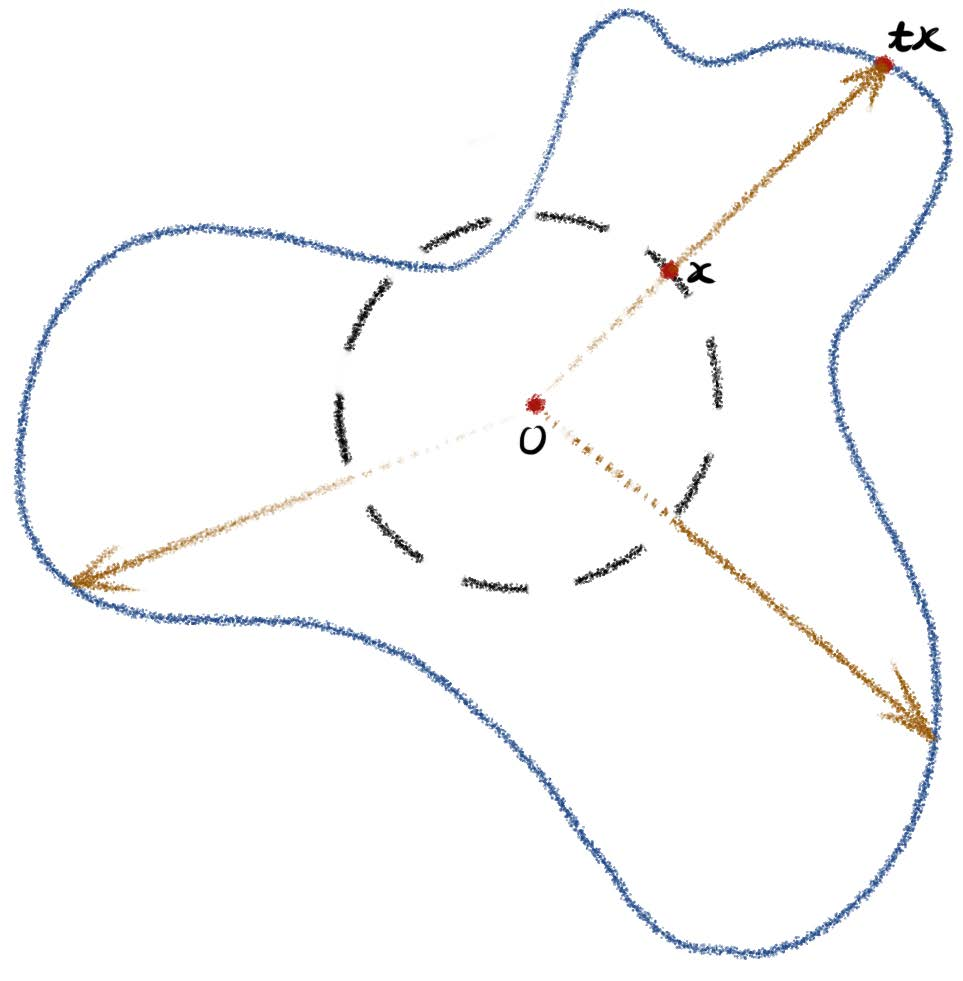
\includegraphics[width=0.4\textwidth]{拓扑学-课本.jpg}
    \caption{定理\ref{定理1}中的f}
    \label{定理中的f}
\end{figure}

这个定理其实很好理解,如果我们学过拓扑学的一些知识就会知道,若0不在 $ f  $ 的值域中,那么 $ 0 $ 周围会有一个“洞”,“洞内”的点均不在值域中。但是我们不可能将一个圆盘通过捏泥巴(连续的直观解释)的方式让它里面有洞,所以不可能零点不存在。如果我们相信这个定理,那么我们有如下推论:
\begin{theorem}[Brouwer fixed point theorem]
    任何连续函数 $ f:D^2\rightarrow D^2  $ 都存在不动点。也就是说, $ \exists x\in D^2 $ 使得 $ f(x)=0 $ 
\end{theorem}
\begin{remark}
    我们可以简单的理解这个定理,它其实的意思是:如果我们搅拌一个咖啡杯,我们假定咖啡杯表面的液体分子不会向下走。那么无论我们怎么搅拌,咖啡杯表面总是有一个点与最初的位置相同,这是因为我们搅拌的过程总是连续的。\\
    事实上,这个定理可以拓展到三维领域,因此,我们不需要做任何假设就可以得出一个数学上绝对正确的结论:如果我们在玩一个榨汁机,无论我们怎么在榨汁机里搅拌,榨汁机里总是有一个点与最初的位置相同。这就是拓扑学研究的事情。
\end{remark}
\begin{proof}
    假设 $ f  $ 没有不动点,那么对于任意的 $ x\in D^2 $,  $ f(x)  $ 与 $ x  $ 不是同一个点,因此我们可以画出从 $ f(x) $ 到 $ x  $ 的射线 $ l_x $。设 $ l_x  $ 与单位圆边界 $ S^1 $ 交于点 $ g(x) $。这样我们就构造出了一个函数 $ g:D^2\rightarrow D^2  $, $  x\mapsto g(x) $。\\
    容易验证这几点要求:
    \begin{enumerate}
        \item $ g(x) $ 是连续的。
        \item 对 $ x\in S^1 $, $ g(x) $ 满足 $ g(x)=x $.
        \item  $ g(x)\in S^1 $,故不存在 $ g(x)=0 $.  
    \end{enumerate}  
    但是由定理\ref{定理1}, $ g  $ 满足存在 $ x $,  $ g(x)=0 $。这与上面的第三点矛盾!\\
    这样我们就证明了问题。   
\end{proof}
\begin{figure}[htb]
    \centering
    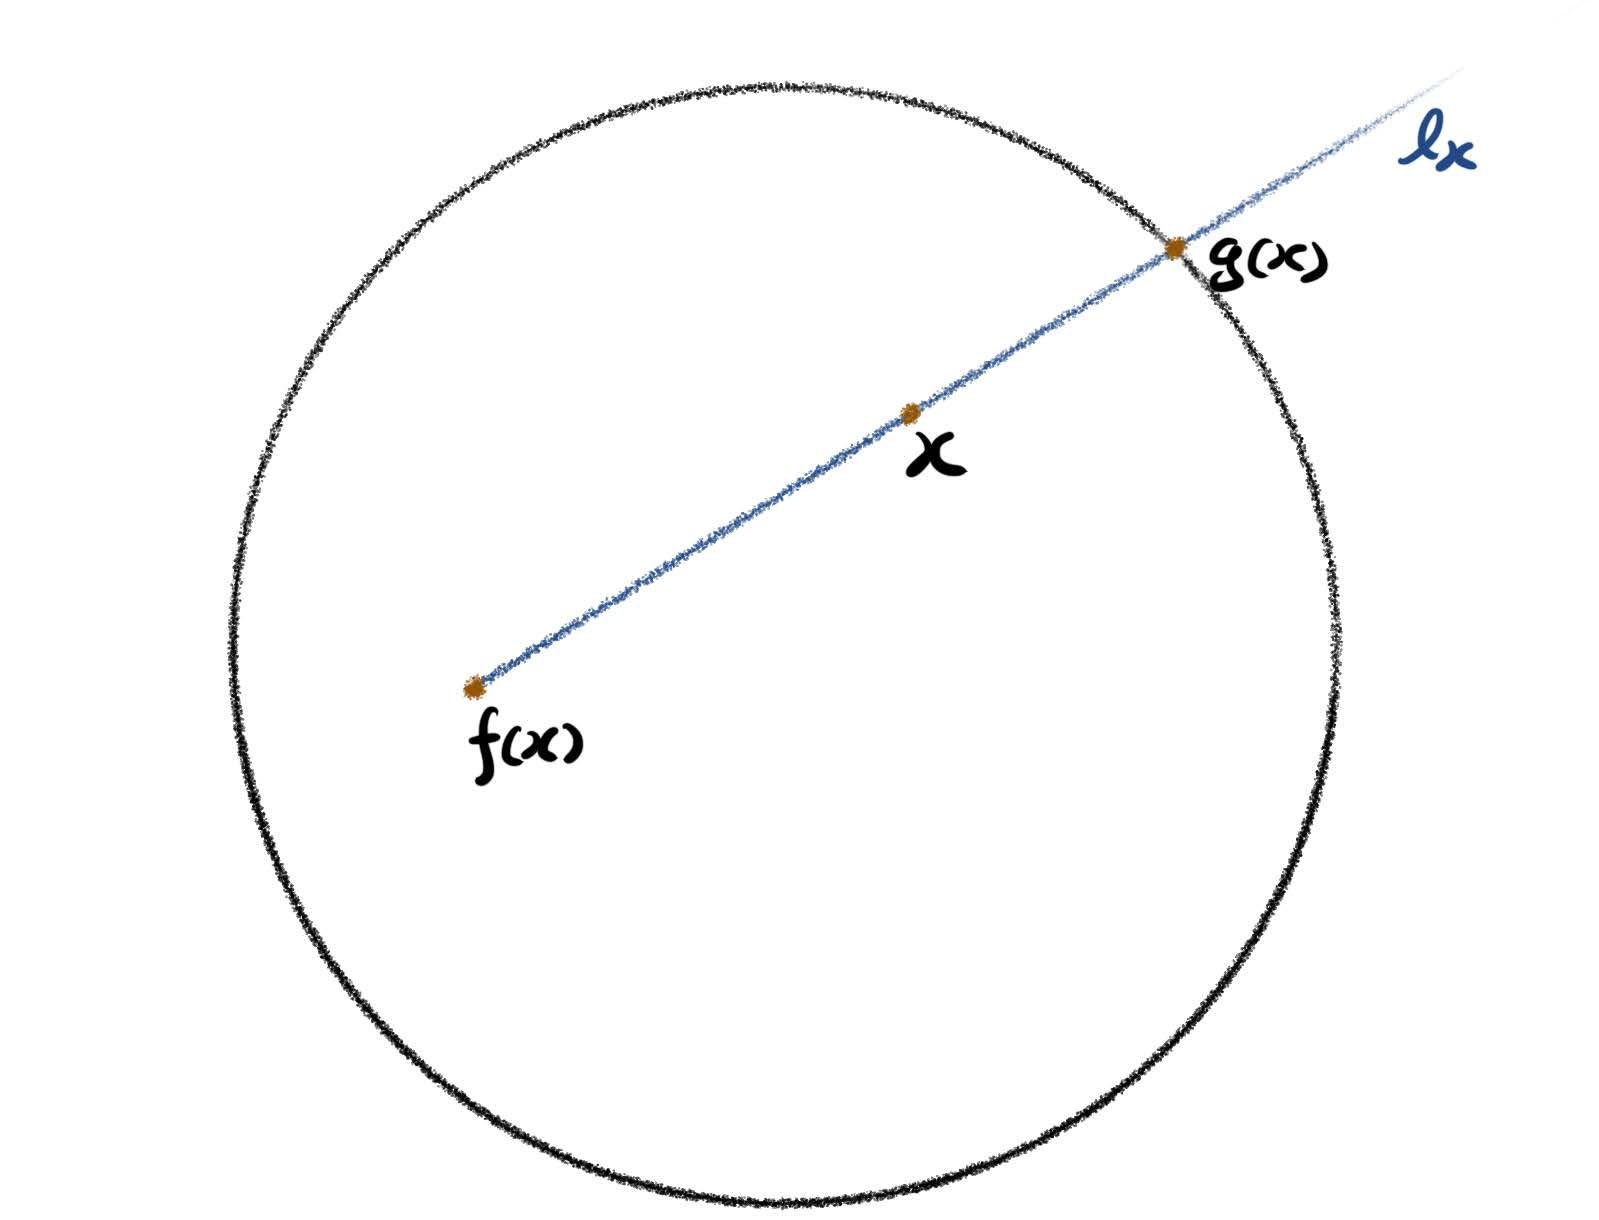
\includegraphics[width=0.4\textwidth]{Brouwer.jpg}
    \caption{$ g(x) $的构造}
    \label{Brouwer定理}
\end{figure}
\begin{remark}
    这个证明非常的漂亮,特别是运用了反证法这一事情,居然有利用反证法证明存在性的方法!尽管这个定理的证明由Brouwer给出,但是他在后期并不承认这个证明。这是数学中非常著名的\textbf{直觉主义}学派,他们宣称,数学的对象只能通过直接证明而不能通过反证法。因此存在性证明必须是构造性的。这从这个定理中也可以理解:你证明了不存在不动点是有问题的,但却完全不能描述它的大概位置。那么凭什么认为这个无中生有的不动点存在呢。
\end{remark}

笔者介绍了一个拓扑学中的经典例子和直觉主义学派作为本节的引言部分,目的是想让读者们了解数学的概念是不断的抽象的过程,例如我们可以用连续函数去描述搅拌咖啡机的起始点到终点。拓扑学就是这样一个学科,本质上是研究多维空间下的“捏娃娃”或者说“搅拌”对于一个对象中的点的影响。图就是一个拓扑对象。\\以及,有关数学的哲学和思想也是不断的与时俱进的。以往的数学家通常都是以“直觉”作为证明的基础,这一思想对现代数学家也有很深远的影响,往往数学家认为idea重要而详细而繁琐的证明不重要。然而我们不得不承认的是,现代数学必须建立在一个“欧几里得”式的严格的公理体系之下,但这个体系每个人往往都有不同的看法,例如直觉主义的观点。\\
有的人也会认为选择公理(我们可以从无穷个非空集合中分别选择出一个元素组成一个集合)是不成立的。这听上去很奇怪,但似乎你也没有一个理由去解释它,特别是当罗素提出罗素悖论后,人们对集合的态度往往很谨慎。\\
我们唯一能做的,就是严谨的研究每一个证明过程,这样认同或不认同的人都能找到适合自己的一个定理。而严谨体现在方方面面,例如“连续”的定义,我们必须对“搅拌”或者“捏娃娃”或者说”连续“的东西的概念作出数学上的定义。而这样的定义也是帮助我们理解这个对象的,例如Brower定理就是这样一个例子,只有严格的定义我们才能更自然地去研究。\\
引言到这里基本结束了,接下来我会引导读者研究数学的方方面面,以材料的形式探讨数学家的思维方式。
\begin{figure}[htb]
    \centering
    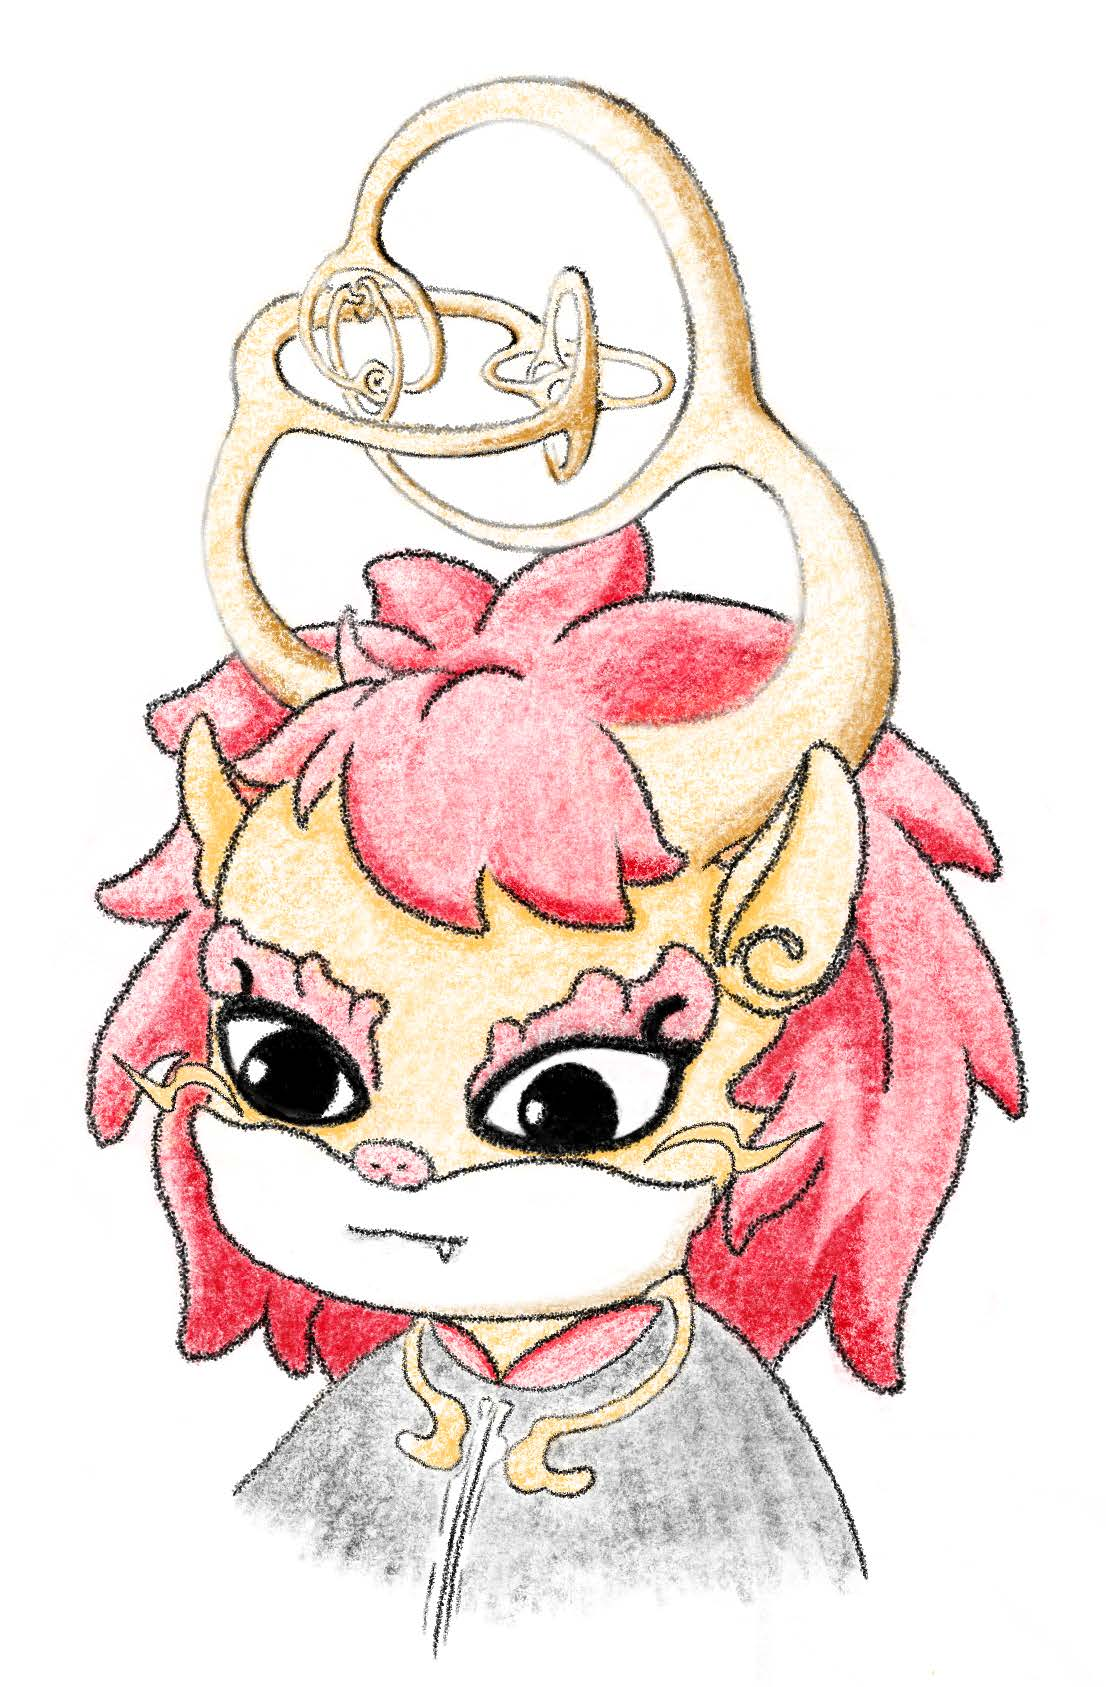
\includegraphics[width=0.5\textwidth]{麒麟.jpg}
    \caption{三维空间中一个外表面封闭的形状内部不一定与外界不连通}
    \label{麒麟图}
\end{figure}
\newpage